\documentclass{article}

% draw flow charts
\usepackage{tikz}
\usetikzlibrary{shapes.geometric, arrows}

% set paper size, orientation and margins
\usepackage[a4paper, portrait, margin=1.5cm]{geometry}

% justify text
\usepackage{ragged2e}
\justifying

% empty lines between paragraphs instead of first line indentation
\usepackage{parskip}

% use \url tag
\usepackage{url}

% clickable links and \nameref
\usepackage{hyperref}

% begin flow chart blocks
\tikzstyle{startstop} = [rectangle, rounded corners,
minimum width=3cm, minimum height=1cm,
text centered, text width=3cm,
draw=black, fill=red!30]

\tikzstyle{io} = [trapezium,
trapezium stretches=true,
trapezium left angle=70,
trapezium right angle=110,
minimum width=3cm, minimum height=1cm,
text centered, text width=3cm,
draw=black, fill=blue!30]

\tikzstyle{process} = [rectangle,
minimum width=3cm, minimum height=1cm,
text centered, text width=3cm,
draw=black, fill=orange!30]

\tikzstyle{decision} = [diamond,
aspect = 2,
minimum width=3cm, minimum height=1cm,
text centered, text width=2.5cm,
draw=black, fill=green!30]
\tikzstyle{arrow} = [thick,->,>=stealth]
% end flow chart blocks

%TITLE INFORMATION

\title{
    Preparing ('Digitizing') Images with Inkscape and Ink/Stitch\\
    for Machine Embroidery}
\author{Harald Kraft}
\date{
    \today
    \bigbreak
    % add license information to title
    This entire document is licensed under the GNU Affero General Public License Version 3.\\
    \url{https://gnu.org/licenses/agpl.html}}

%TITLE INFORMATION

\begin{document}

    \maketitle

    \tableofcontents

    \pagebreak

    \section{Prerequisites / Preparations}
        \subsection{Inkscape}
            The first piece of required software is Inkscape. It can be found at \url{https://inkscape.org/}. The most recent stable version at the time of writing is 1.2.2.
            If your operating system is Windows, make sure to try to download and install the 64-bit version first. If the setup gives you an error directly after starting it, try the 32-bit version second.
            Inkscape is available via the default repositories of almost all Linux distributions. If yours should be the exception, you can use the available Appimage or Snap Store images.
            For MacOS please make sure to select the correct version for older systems with Intel or newer system with Apple M processors.

        \subsection{Ink/Stitch}

            Ink/Stitch is a plugin (addition) for Inkscape. It can only run, if you already have a working Inkscape installation. Ink/Stitch can be found here: \url{https://inkstitch.org/}
            To install the plugin correctly, please follow the Instructions that can be found here: \url{https://inkstitch.org/docs/install/}. Please select your operating system accordingly.

        \subsection{Using Ink/Stitch}

            To access the additional functionality that Ink/Stitch offers, open Inkscape and click on 'Plugin' $\rightarrow$ 'Inkstitch'.
            Ink/Stitch will be essential in preparing and exporting our embroidery files. Nevertheless, besides the functionality the plugins offers, we will also require many functions that are already included in Inkscape.
            Knowing or learning how Inkscape works there will help quite a bit in creating beautiful embroideries.
            To get to know how Inkscape beyond what this document will teach you, you can find a lot of help on the Inkscape website. Alternatively you can look for introductory videos and tutorials on many platforms like Youtube.
            \smallbreak
            The following pages will try to explain the necessary steps to create an embroidery pattern from an image file.

        \subsection{Setting up Inkscape}
        %TODO: set up grid and hoop sizes

        \subsection{Useful Resources for learning Inkscape and Ink/Stitch}

        Inkscape:\newline
        A vast collection of introductions and tutorials on how to do almost anything in Inkscape can be found on \href{https://inkscape.org/learn/}{the applications homepages learning section}.

        Ink/Stitch:\newline
        A good tutorial on many things you need to know about the usage of Ink/Stitch, stitch types, creating and editing embroidery motives and more can be found in the \href{https://inkstitch.org/docs/customize/}{Ink/Stitch Manual on the projects homepage}.
        It even contains a short introduction into Inkscape. There you can click on the sections on the left to go to parts that you want to learn more about.

    \pagebreak

    \section{Workflow}
        \subsection{Overview}
            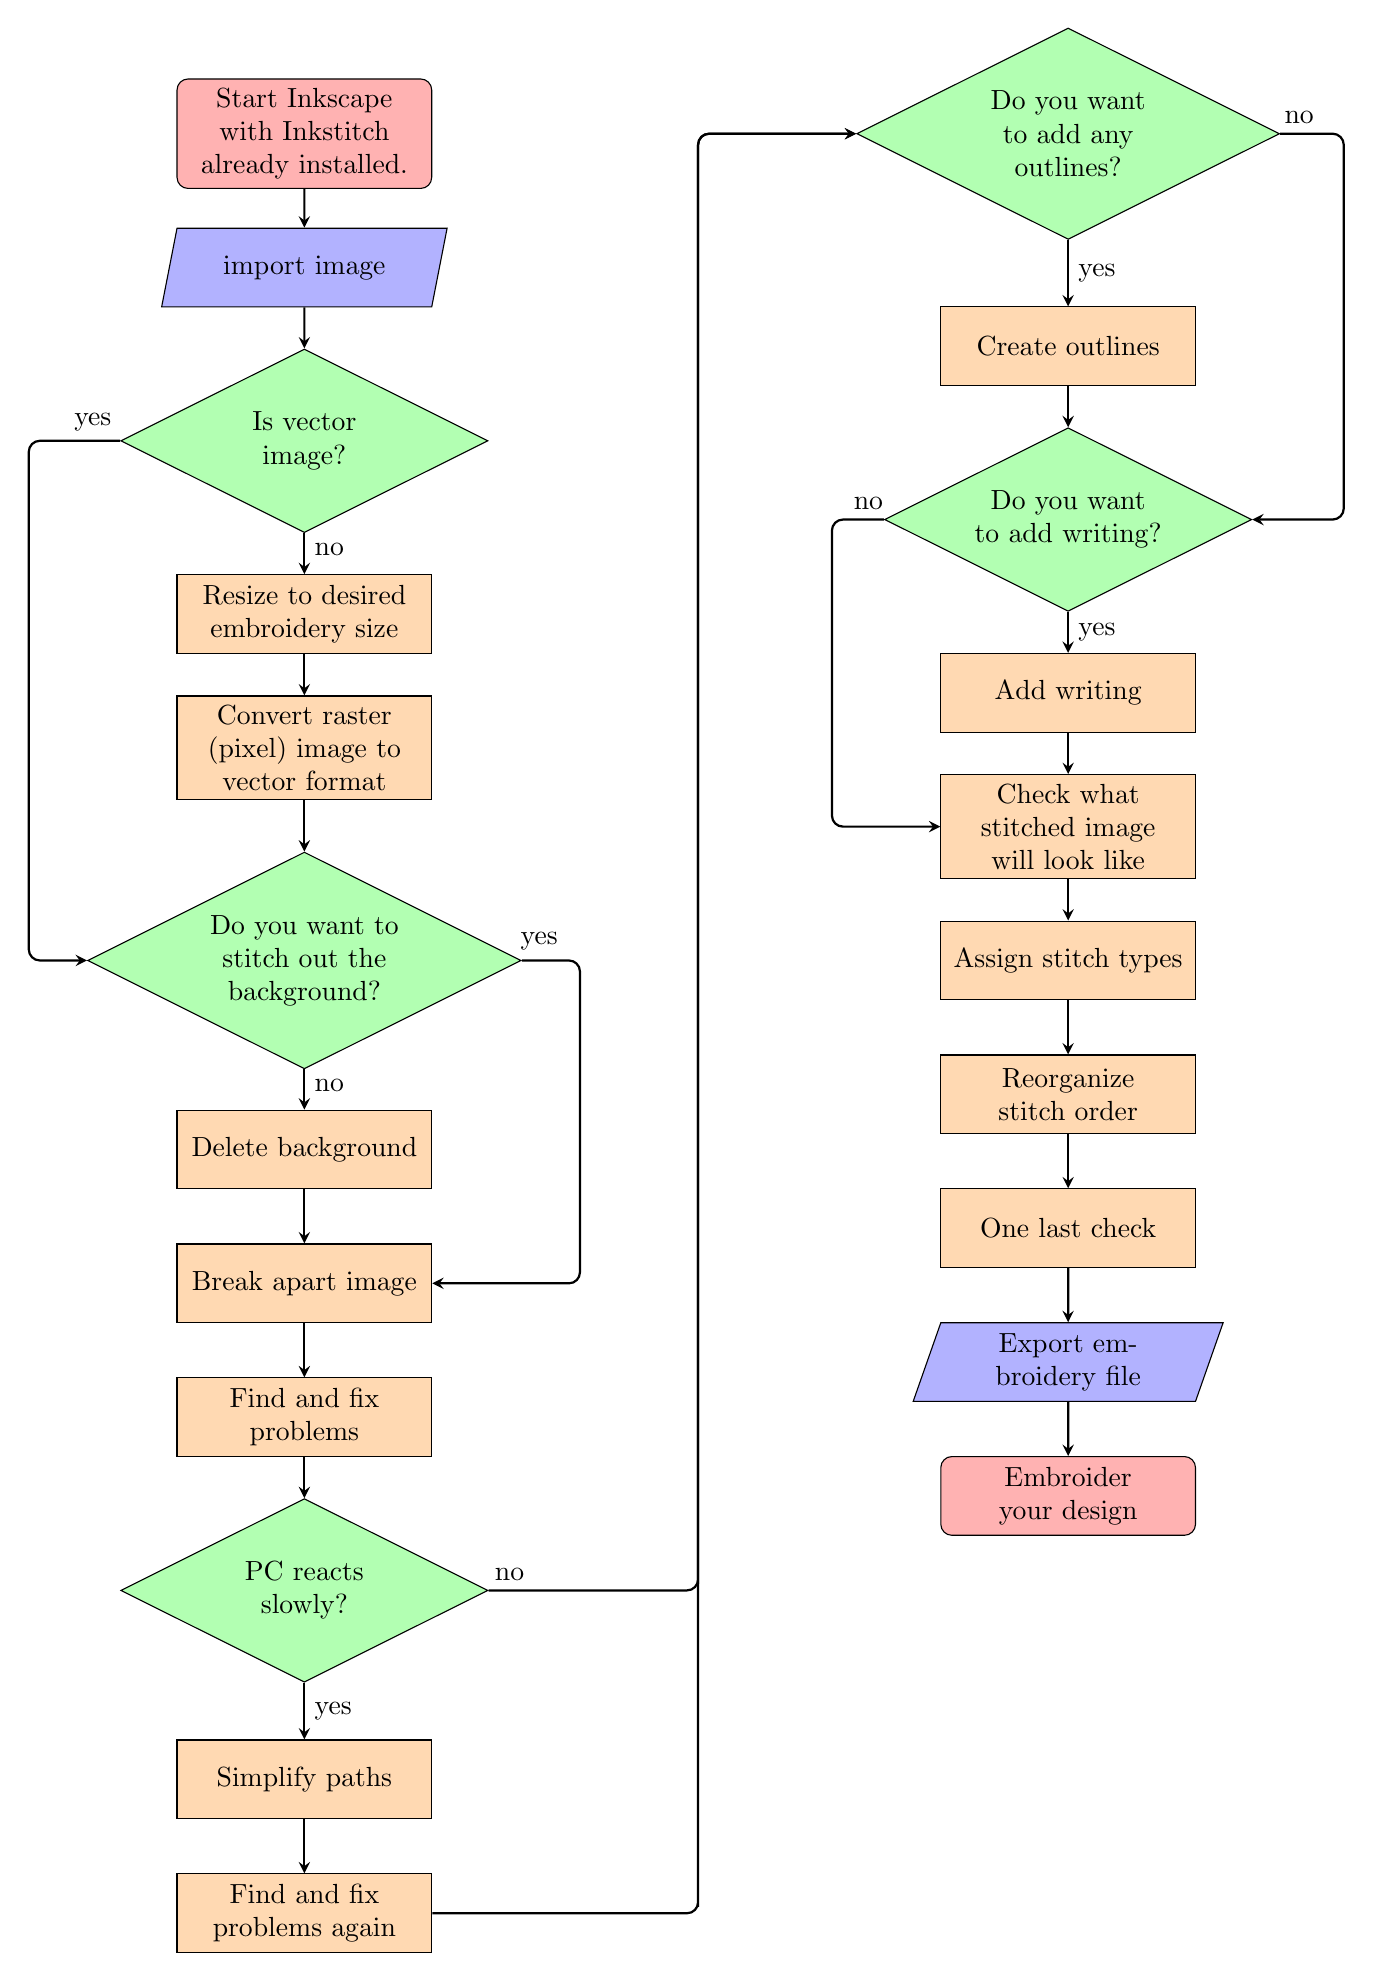
\begin{tikzpicture}[node distance=1.7cm]
                \node (start) [startstop] {Start Inkscape with Inkstitch already installed.};
                \node (import) [io, below of=start] {import image};
                \node (isVector) [decision, below of=import, yshift=-0.5cm] {Is vector image?};
                \node (resize) [process, below of=isVector, yshift=-0.5cm] {Resize to desired embroidery size};
                \node (conv) [process, below of=resize] {Convert raster (pixel) image to vector format};
                \node (backgr) [decision, below of=conv, yshift=-1cm] {Do you want to stitch out the background?};
                \node (delBackgr) [process, below of=backgr, yshift=-0.7cm] {Delete background};
                \node (split) [process, below of=delBackgr] {Break apart image};
                \node (trouble) [process, below of=split] {Find and fix problems};
                \node (slow) [decision, below of=trouble, yshift=-0.5cm] {PC reacts slowly?};
                \node (simplify) [process, below of=slow, yshift=-0.7cm] {Simplify paths};
                \node (troubleAgain) [process, below of=simplify] {Find and fix problems again};
                \node (wantOutlines) [decision, right of=start, xshift=8cm] {Do you want to add any outlines?};
                \node (outlines) [process, below of=wantOutlines, yshift=-1cm] {Create outlines};
                \node (wantLettering) [decision, below of=outlines, yshift=-0.5cm] {Do you want to add writing?};
                \node (lettering) [process, below of=wantLettering, yshift=-0.5cm] {Add writing};
                \node (check) [process, below of=lettering] {Check what stitched image will look like};
                \node (types) [process, below of=check] {Assign stitch types};
                \node (order) [process, below of=types] {Reorganize stitch order};
                \node (lastCheck) [process, below of=order] {One last check};
                \node (export) [io, below of=lastCheck] {Export embroidery file};
                \node (embroider) [startstop, below of=export] {Embroider your design};


                \draw [arrow] (start) -- (import);

                \draw [arrow] (import) -- (isVector);

                \draw [arrow] (isVector) -- node[pos=0.4, right] {no} (resize);
                \draw [arrow, rounded corners=4pt] (isVector) -- ++ (-3.5,0) node[pos=0.3, above] {yes} |- (backgr);

                \draw [arrow] (resize) -- (conv);

                \draw [arrow] (conv) -- (backgr);

                \draw [arrow] (backgr) -- node[pos=0.4, right] {no} (delBackgr);
                \draw [arrow, rounded corners=4pt] (backgr) -- ++ (3.5,0) node[pos=0.3, above] {yes} |- (split);

                \draw [arrow] (delBackgr) -- (split);

                \draw [arrow] (split) -- (trouble);

                \draw [arrow] (trouble) -- (slow);

                \draw [arrow] (slow) -- node[pos=0.5, right] {yes} (simplify);
                \draw [arrow, rounded corners=4pt](slow) -| ++ (5,0) node[pos=0.05, above] {no} |- (wantOutlines);

                \draw [arrow] (simplify) -- (troubleAgain);

                \draw [arrow, rounded corners=4pt] (troubleAgain) -| ++ (5,0) |- (wantOutlines);

                \draw [arrow] (wantOutlines) -- node[anchor=west] {yes} (outlines);
                \draw [arrow, rounded corners=4pt] (wantOutlines) -- ++ (3.5,0) node[pos=0.3, above] {no} |- (wantLettering);

                \draw [arrow] (outlines) -- (wantLettering);

                \draw [arrow] (wantLettering) -- node[anchor=west] {yes} (lettering);
                \draw [arrow, rounded corners=4pt] (wantLettering) -- ++ (-3,0) node[pos=0.3, above] {no} |- (check);

                \draw [arrow] (lettering) -- (check);

                \draw [arrow] (check) -- (types);

                \draw [arrow] (types) -- (order);

                \draw [arrow] (order) -- (lastCheck);

                \draw [arrow] (lastCheck) -- (export);

                \draw [arrow] (export) -- (embroider);
            \end{tikzpicture}

        \pagebreak

        \subsection{Import Image}

            To import an image into Inkscape you multiple options. Three of these are:

            \begin{itemize}
                \item Directly open the image with Inkscape.
                \item Drag the image file from an file explorer window into the Inkscape window.
                \item In Inkscape click on 'File' $\rightarrow$ 'Import' and select the file you would like to import.
            \end{itemize}

            When importing an image, Inkscape might display an import dialogue which lets you select certain file format specific options.
            Usually it is sufficient to leave these options at their default values and just confirm the dialogue.

        \subsection{File Types}

            There are two fundamentally different classes of file formats:
            \begin{itemize}
                \item \textbf{vector} formats like \textbf{SVG, EPS, AI, PDF} (is often used as a container for vector formats), etc.
                \item \textbf{raster} (pixel) formats like \textbf{JP(E)G, PNG, WEBP, GIF, TIFF, BMP}, etc.
            \end{itemize}

            \subsubsection{Vector Formats}

                Vector images are comprised of shapes an strokes.
                This means that they usually can be scaled to pretty much every size without loosing visual quality.

                That also means that editing them may be a lot easier or a bit harder than editing images that are made out of pixels.
                In any case, if you have never worked with vector images, it may take a little bit of time to get used to it.

            \subsubsection{Raster Formats}

                Raster image formats, often better known as pixel formats, build up the image from square pixels. It is therefore impossible to edit shapes, lines, text or any other type of the images content directly.
                Manipulating such an image after the fact is there very often much more labour intensive. On the other hand, most images found on the internet and all images exported by digital cameras are raster images.

                Ink/Stitch is only able to handle vector images. Therefore, in chapter \ref{vectorConversion} \nameref{vectorConversion} we will learn how to convert a raster image to a vector format.
                This has the added benefit of being able to manipulate the image in many ways that would be impossible or very difficult with a raster image.

        \subsection{Resizing}

        It is often a good idea to resize your image to roughly the size that your finished embroidery pattern is supposed be.
        You even can set up Inkscape so that it will display images at the right size when scaling is set to 100\%. For that, go to the 'Preferences' $\rightarrow$ 'Interface'.
        Inkscape will show a ruler that you can compare to another, physical ruler. You can select the correct measurement unit for your physical ruler to the right of Inkscapes ruler. Then adjust the slider above until your and Inkscapes ruler match as exactly as possible.
        Make sure to also check the box 'Show zoom percentage corrected by factor'.

        To resize an image after importing it into Inkscape, follow these steps:
        Enable the 'Select and transform' tool by clicking on the topmost arrow in the standard too bar or by pressing 'S' on your keyboard.
        Then, click on the image you would like to resize. You can now drag one of the images corner to change the size or enter the desired dimensions in the 'W' and 'H' boxes at the top of the screen.
        To keep the aspect ratio the same as the original image hold the 'CTRL' key while dragging a corner or click the lock icon between the 'W' and 'H' boxes before entering a new size.
        You can change the measurement unit by clicking the drop down menu to the right of the 'H' box.

        \subsection{Conversion to Vector Image} \label{vectorConversion}
        %TODO: Trace Bitmap

        \subsection{Delete Background}
        %TODO

            \subsubsection{Delete Background Layer}
            %TODO

            \subsubsection{Delete "Holes"}
            %TODO

        \subsection{Break Apart Image}
        %TODO

        \subsection{Finding and fixing Problems}
        %TODO

            \subsubsection{Troubleshooter}
            %TODO

            \subsubsection{Clean up Document}
            %TODO

            \subsubsection{Small Infill}
            %TODO

            \subsubsection{Border Crosses Itself}
            %TODO

            \subsubsection{Rung mIntersects Rail more than Once (Satin Stitch)}
            %TODO

        \subsection{Simplify Paths}
        %TODO

        \subsection{Finding and Fixing Problems, Again}
        %TODO

        \subsection{Creating Outlines}
        %TODO

        \subsection{Adding Writing / Lettering}
        %TODO

        \subsection{Checking what the Stitched Image will look like}
        %TODO

        \subsection{Assigning Stitch Types}
        %TODO

            \subsubsection{Straight Stitch}
            %TODO

            \subsubsection{Satin Stitch}
            %TODO

            \subsubsection{Fill Stitch}
            %TODO

        \subsection{Reorganizing the Stitch Order}
        %TODO

            \subsubsection{Grouping same Colour Parts}
            %TODO

            \subsubsection{Avoiding visible Jump Stitches}
            %TODO

        \subsection{One last Check}
        %TODO

        \subsection{Exporting to a File your Embroidery Machine can understand}
        %TODO

\end{document}
